\begin{sloppypar*}
    
    \begin{figure}
        \centering
        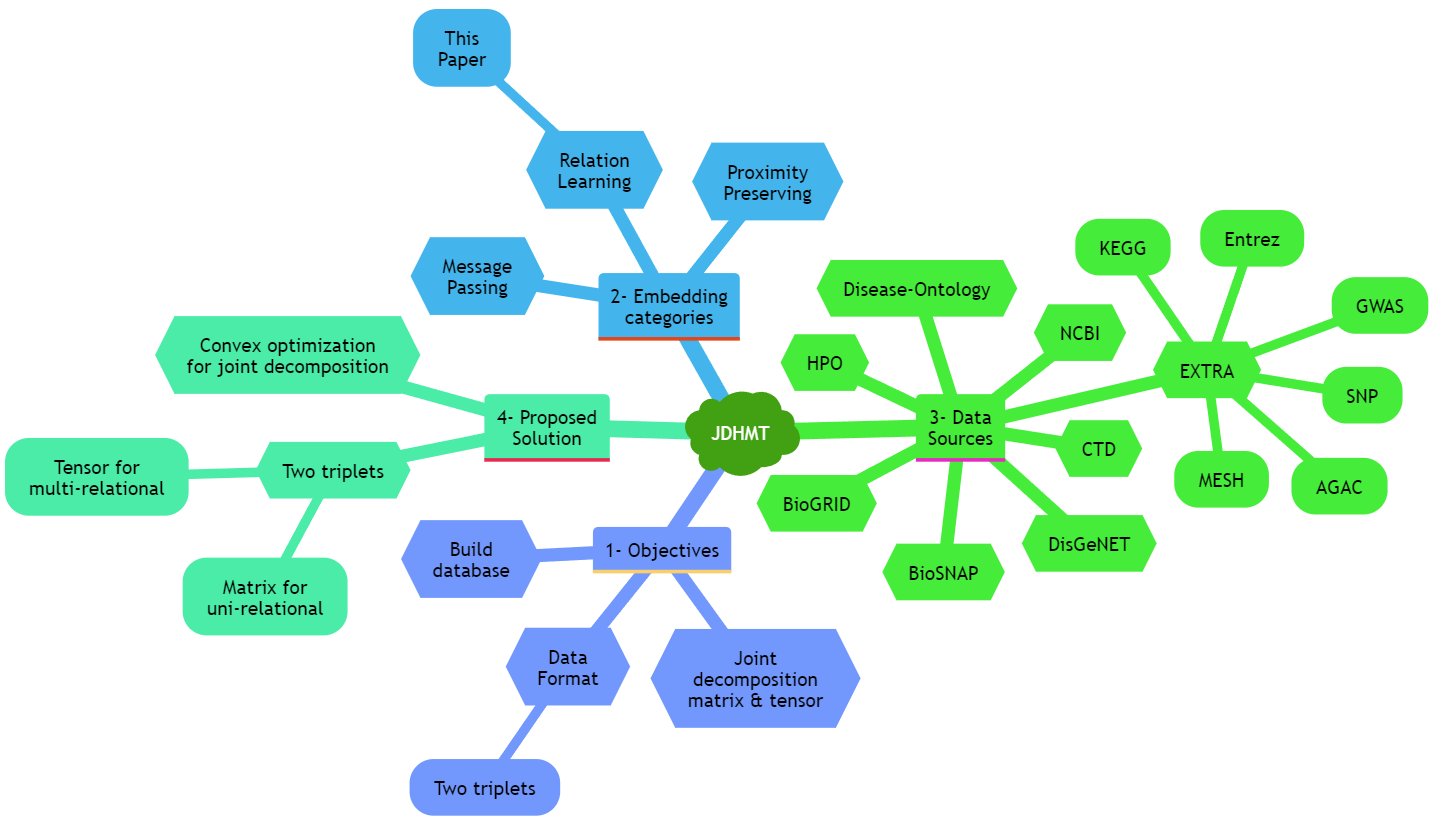
\includegraphics[width=170mm,scale=1]{mindmap.png}
        \caption{Mindmap}
        \label{fig:mindmap}
    \end{figure}

    Identifying genes that contribute to a disease can further our understanding
    in human \textbf{physiology}, \textbf{pathology} and thus enable better
    research in \textbf{pharmacology}. In this paper, the authors have setup a
    heterogeneous graph of \textit{genes} and \textit{diseases} and utilised the
    techniques of graph embedding (DeepWalk $+$ word2vec) followed by GCN \cite{kipfGCN}
    to learn embeddings for both the \textit{gene nodes} and the \textit{diseases
    nodes}. This is followed by a decoder module which learns to predict the
    probability of association between any \textit{gene-disease} pair. An overview
    of all the components of the paper is summarised in the \textit{mindmap} in
    Figure \ref{fig:mindmap}.
\end{sloppypar*}